\chapter{Basic Constructions with Ruler and Compass}

\section{Defining lines, circles and the set of constructable points}
First we need to define what construction using a ruler and compass means.
We will use $\mathbb{C}$ as plane of drawing and $\mathcal{M} \subset \mathbb{C}$ as the set of constructed points.

\begin{definition}[Line]
    \label{def:line}
    \lean{Construction.line}
    \leanok
    A line $L := (x,y)$ is defined by two points $x,y\in\mathbb{C}$ with $x\ne y$ and a set $$l:=\{\lambda x+(1-\lambda)y\mid\lambda\in\mathbb{R}\}.$$
    We say two lines are equal if their generated set is equal.
\end{definition}
\begin{remark}
    To express lines in the most general way, they are stated without the requirement that $x\ne y$, which allows for trivial lines. 
    The condition is only included in the lemmas that require it.
\end{remark}


\begin{definition}[Circle]
    \label{def:circle}
    \lean{Construction.circle}
    \leanok
    A circle $C := (c,r)$ is defined by a center $c$ with  $c\in\mathbb{C}$, a radius $r\in\mathbb{R}_{\ge 0}$ and the set: $$c:=\{z\in\mathbb{C} \mid\|z-c\|=r\}.$$ 
    We say a circle is if the underlying set is equal.
\end{definition}

\begin{lemma}
    \label{lem:circle_not_eq_iff}
    \lean{Construction.circle_not_eq_iff, Construction.circle_not_eq_iff_radius}
    \leanok
    \uses{def:circel}
    If we have two circles $C_1 = (c_1,r_1)$, $C_2 = (c_2,r_2)$ and we have $c_1 \ne c_2$ or $r_1  \ne r_2 $ then the circles aren't equal. 
\end{lemma}


\begin{definition}[Set of lines]
    \label{def:set_of_lines}
    \lean{Construction.L, Construction.l_in_L_M}
    \leanok
    \uses{def:line}
    $\mathcal{L(M)}$ is the set of all real straight lines $l$, with $| l\cap \mathcal{M} |\ge 2$. As a set this is:
    \begin{equation*}
        \mathcal{L(M)} := \{l \mid l = \{x,y\} \text{ with }x,y \in \mathcal{M} \land x \neq y\}.
    \end{equation*}
\end{definition}

\begin{definition}[Set of circles]
    \label{def:set_of_circles}
    \lean{Construction.C, Construction.c_in_C_M}
    \leanok
    \uses{def:circle}
    $\mathcal{C(M)}$ is the set of all circles in $\mathbb{C}$, with center in $\mathcal{M}$ and radius of $\mathcal{C}$ which is the distance of two points in $\mathcal{M}$. As an equation this is:
    $$\mathcal{C(M)}:=\{c\mid c = \langle c, \dist r_1 r_2 \rangle \text{ with } c,r_1,r_2\in M\}.$$
\end{definition}

\begin{definition}[Rules to construct a point]
    \label{def:rules_to_constructed_a_point}
    \lean{Construction.ill,Construction.ilc,Construction.icc,Construction.ICL_M}
    \leanok
    \uses{def:set_of_lines, def:set_of_circles}
    We define operations that can be used to construct new points.
    \begin{enumerate}
        \item $(ILL)$ is the intersection of two different lines in $\mathcal{L(M)}$.
        \item $(ILC)$ is the intersection of a line in $\mathcal{L(M)}$ and a circle in $\mathcal{C(M)}$.
        \item $(ICC)$ is the intersection of two different circles in $\mathcal{C(M)}$.
    \end{enumerate}
    $ICL(\mathcal{M})$ is the union of all points that can be constructed using the operations $(ILL)$, $(ILC)$ and $(ICC)$ and $\mathcal{M}$.
\end{definition}

\begin{definition}[Set of constructable points]
    \label{def:set_of_constructable_points}
    \lean{Construction.M_I,Construction.M_inf}
    \leanok
    \uses{def:rules_to_constructed_a_point}
    We inductively define the chain
    \begin{equation*}
        \mathcal{M}_0 \subseteq \mathcal{M}_1 \subseteq \mathcal{M}_2 \subseteq \dots
    \end{equation*}
    with $\mathcal{M}_0 = \mathcal{M}$ and $\mathcal{M}_{n+1} = ICL(\mathcal{M}_n)$\newline
    and call $\mathcal{M}_{\infty} = \bigcup_{n \in \mathbb{N}} \mathcal{M}_n$ the set of all constructable points.
\end{definition}

\begin{remark}
    The set of lines, circles and their intersection $icc$, $ilc$, $icc$ are monoton, i.e. for $N\subseteq M$ is $\mathcal{L(N)}
    \subseteq\mathcal{L(M)}$,\dots .
\end{remark}

\section{Properties of Lines}
In light of the fact that a considerable proportion of the forthcoming project will entail the manipulation of lines and the absence of an existing formalisation from MathLib, 
it is imperative to illustrate the fundamental properties that will be utilised throughout the remainder of the project.

\begin{lemma} 
    \label{lem:line_pionts_iff}
    \lean{Construction.line_pionts_iff}
    \leanok
    \uses{def:line}
    The set of points of a line $l$ is not defined by one position vector, i.e. for every $\alpha\in l$  $\{\lambda x+(1-\lambda)y\mid\lambda\in\mathbb{R}\} = \{\lambda x+\lambda y+\alpha\mid\lambda\in\mathbb{R}\}$.
\end{lemma}
\begin{proof}
    Two sets are equal if they have the same elements. 
    Since $\alpha$ is in $l$, there exists a $\lambda_{\alpha}$ such that $\alpha = \lambda_{\alpha} x+(1-\lambda_{\alpha})y$.
    
    "$\Rightarrow:$" Let $z=\lambda_0 x + (1-\lambda_0)y$ (i.e.  $z\in\{\lambda x+(1-\lambda)y\mid\lambda\in\mathbb{R}\}$), we have to show that $z\in \{\lambda x+\lambda y+\alpha\mid\lambda\in\mathbb{R}\}$,
    which is equivalent to the existence of $\lambda$ such that $z = \lambda x+\lambda y+\alpha$. If we use $\lambda = \lambda_0 - \lambda_{\alpha} $ we get
    $$(\lambda_0 - \lambda_{\alpha}) x + ((\lambda_0 - \lambda_{\alpha}))y + \alpha  \overset{\alpha = \lambda_{\alpha} x+(1-\lambda_{\alpha})y}{=} \lambda_0 x - \lambda_0 y + y = z$$ % \lambda_{\alpha} x+(1-\lambda_{\alpha})y + (\lambda_0 - \lambda_{\alpha}) x + ((\lambda_0 - \lambda_{\alpha}))y
    $\Leftarrow:$ Let $z$ be in $\{\lambda x+(\lambda)y+\alpha\mid\lambda\in\mathbb{R}\}$, if we use $\lambda = \lambda_0 + \lambda_{\alpha} $ we get
    $$(\lambda_0 + \lambda_{\alpha}) x + (1 -(\lambda_0 + \lambda_{\alpha}))y = \lambda_0 x - \lambda_0 y + \lambda_{\alpha} x - \lambda_{\alpha} y + y \overset{\alpha = \lambda_{\alpha} x+(1-\lambda_{\alpha})y}{=}  \lambda_0 (x - y) + \alpha = z$$
\end{proof}

\begin{definition}[parallel]
    \label{def:parallel}
    \lean{Construction.parallel}
    \leanok
    \uses{def:line}
    Two lines $l_1$ and $l_2$ are parallel if they have the same slope, i.e. $\exists r\in\C: l_1 = \{x + r \mid x\in l_2\}$.
\end{definition}

\begin{lemma}[Parallel defined by basis]
    \label{lem:parallel_by_basis}
    \lean{Construction.parallel_basis}
    \leanok
    \uses{def:line, def:parallel}
   If the basis of two lines is moved by the same amount, i.e $l_1.z_1 - l_2.z_1 = l_1.z_2- l_2.z_2$, then they are parallel.
\end{lemma}
\begin{proof}
    \uses{def:line, def:parallel}
    We have to lines $l_1, l_2$ with basis $z_1, z_2$ and $l_1.z_1 - l_2.z_1 = l_1.z_2- l_2.z_2$. To show that they are parallel we have to show that $$\exists r: l_1 = \{z + r \mid z\in l_2\}.$$
    To make it easier to read we define $a := l_1.z_1$, $b:= l_1.z_2$, $x:= l_2.z_1$ and $y:= l_2.z_2$.\\
    Upon unravelling the definition, it becomes evident that we need to show that  $\exists t: t \cdot a +(1-t)\cdot b=z \iff \exists s :s \cdot x+(1-s)y+(a-x)=z$.\\
    $\Rightarrow:$ Claim $s = \frac{t(a-b)}{x-y}$ is a solution.\\
    \begin{proof}
    \begin{align*}
        && z &= s \cdot x+(1-s)y+(a-x)&&| z= t\cdot a+(1-t)\cdot b\\
        &\Leftrightarrow & t\cdot a+(1-t)\cdot b  &= s \cdot x+(1-s)y+(a-x)\\
        &\Leftrightarrow & t\cdot a-t\cdot b +b &= s \cdot x-s\cdot y + y+(a-x)&& | -y\\
        &\Leftrightarrow & t\cdot a-t\cdot b + b-y  &= s \cdot x-s\cdot y+(a-x)-y&&| a-x =b-y\\
        &\Leftrightarrow & t\cdot a-t\cdot b  &= s \cdot x+s\cdot y\\
        &\Leftrightarrow & t(a-b)  &= s(x-y)&&|s:= \frac{t(a-b)}{x-y}\\
        &\Leftrightarrow & t(a-b)  &= \frac{t(a-b)}{x-y}(x-y)\\
        &\Leftrightarrow & t(a-b)  &= t(a-b)
    \end{align*}
    \end{proof}
    "$\Leftarrow:$" Claim $t = \frac{s(x-y)}{a-b}$ is a solution.
    \begin{proof}
    \begin{align*}
        && t\cdot a+(1-t)b &= z&&| z:= s \cdot x+(1-s)y+(a-x)\\
        &\Leftrightarrow& t\cdot a-t\cdot b+b &= s \cdot x-s\cdot y+y+(a-x)&&|-y;a-x =b-y\\
        &\Leftrightarrow& t(a-b) &= s(x-y)&&|t:= \frac{s(x-y)}{a-b}\\
        &\Leftrightarrow& \frac{s(x-y)}{a-b}(a-b) &= s(x-y)
    \end{align*}
    \end{proof}
\end{proof}

\begin{definition}
    \label{def:direction_vector}
    \lean{Construction.direction_vector}
    \leanok
    \uses{def:line}
    The direction vector of a line $l$ is the vector $l.z_1 - l.z_2$.
\end{definition}

\begin{definition}
    \label{def:parallel'}
    \lean{Construction.parallel'}
    \leanok
    \uses{def:line, def:direction_vector}
    Two lines $l_1$ and $l_2$ are \emph{parallel'} if there exists a $k$ such that $l_1.z_1 - l_1.z_2 = k \cdot (l_2.z_1 - l_2.z_2)$.
\end{definition}

\begin{lemma}[Parallel imp parallel']
    \label{lem:parallel_iff_parallel'}
    \lean{Construction.parallel_iff_parallel'}
    \leanok
    \uses{def:parallel, def:parallel'}
    If two lines $l_1$ and $l_2$ are parallel' they are parallel.
\end{lemma}
\begin{remark}
    The other direction holds as well, but is not needed.
\end{remark}

\begin{proof}
    \uses{def:line, def:direction_vector, def:parallel, def:parallel'}
    Let $l_1$ and $l_2$ be two lines with $l_1.z_1 - l_1.z_2 = k \cdot (l_2.z_1 - l_2.z_2)$.
    We have to show that $l_1 = \{z + r \mid z\in l_2\}$, i.e. $\exists r: l_1 = \{z + r \mid z\in l_2\}$.\\
    First we remark that $k\ne 0$ since $l_1.z_1\ne l_1.z_2$. We define $r:= y_1 - y_2$ and show that $l_1 = \{z + r \mid z\in l_2\}$.
    For $z$ to be in $l_1$ is equivalent to $z = \lambda x_1 + (1-\lambda)y_1$ for some $\lambda_0$. 
    For $z$ to be in $\{x + y_1-y_2 \mid z\in l_2\}$  is wquivalent to the existence of $\lambda$ such that 
    $$z = \lambda x_2 + (1-\lambda)y_2 + y_1 - y_2 = \lambda (x_2 - y_2) + y_1 \overset{\lambda = \lambda_0 * k}{=} \lambda_0 k (x_2-x_2)-y_1\overset{x_1-y_1=k(x_2-y_2)}{=}\lambda_0(x_1-y_1)+y_1.$$
\end{proof}

\begin{lemma}[Parallel imp equal]
    \label{lem:eq_of_parallel}
    \lean{Construction.eq_of_parallel}
    \leanok
    \uses{def:line, def:parallel'}
    If two lines $l_1$ and $l_2$ are parallel' and intersect, then they are equal.
\end{lemma}

\begin{proof}
    \uses{def:line, def:parallel', def:direction_vector, lem:line_pionts_iff}
    Let $z\in l_1 \cap l_2$. Then we use lemma \ref{lem:line_pionts_iff} to get $l_1 = l_2 \Leftrightarrow \{\lambda (x_1-y_1)\mid\lambda\in\mathbb{R}\} = \{\lambda (x_2- y_2)+z\mid\lambda\in\mathbb{R}\}$.
    Since for every $\lambda$ we have $\lambda (x_1-y_2) + x = \lambda \cdot k(x_2- y_2)+z$ we get $l_1 = l_2$.
 \end{proof}

\section[The set of constructable points]{The Set $M_{\infty}$}\label{set_of_constructable_points}
In order to work with the set of constructable points, it is necessary to have some basic lemmas at one's disposal. 
While these may appear to be trivial on paper, they are invaluable when undertaking a formalisation.

\begin{lemma}[$\mathcal{M}\subseteq ICL(\mathcal{M})$]
    \label{lem:M_in_ICL_M}
    \lean{Construction.M_in_ICL_M}
    \leanok
    \uses{def:rules_to_constructed_a_point}
    Every set $M$ is included in the constructable points of $M$, i.e.
    \[M \subseteq ICL(M)\]
\end{lemma}
\begin{proof}
    Follows from the definition of $ICL(M)$.
\end{proof}

\begin{lemma}[$\mathcal{M}_i$ Monoton]
    \label{lem:M_i_monoton}
    \lean{Construction.M_I_Monotone,Construction.M_I_Monotone_elm,Construction.M_I_Monotone', Construction.M_I_Monotone_elm'}
    \leanok
    \uses{def:set_of_constructable_points}
    The set $\mathcal{M}_i$ is monoton, i.e. $$\mathcal{M}_i \subseteq \mathcal{M}_{i+1}.$$
    This can be generalised to $$\forall m :\forall n\le m : \mathcal{M}_n \subseteq \mathcal{M}_m.$$
\end{lemma}
\begin{proof}
    Follows from the definition of $\mathcal{M}_i$.
\end{proof}

\begin{lemma}[$\mathcal{M}$ in $\mathcal{M}_i$]
    \label{lem:M_in_Mi}
    \lean{Construction.M_in_M_I }
    \leanok
    \uses{def:set_of_constructable_points}
    The set $\mathcal{M}$ is in $\mathcal{M}_i$, i.e. $$\mathcal{M} \subseteq \mathcal{M}_i.$$
\end{lemma}
\begin{proof}
    \uses{lem:M_i_monoton}
    Combining the fact that $\mathcal{M}_0 = \mathcal{M}$ \ref{def:set_of_constructable_points} and the monotonity of $\mathcal{M}_i$ \ref{lem:M_i_monoton} we get the result.
\end{proof}

\begin{lemma}[$\mathcal{M}_i$ in $\mathcal{M}_{\infty}$]
    \label{lem:M_i_in_M_inf}
    \lean{Construction.M_I_in_M_inf,Construction.M_I_in_M_inf_elm}
    \leanok
    \uses{def:set_of_constructable_points}
    The set $\mathcal{M}_i$ is in $\mathcal{M}_{\infty}$, i.e. $$\mathcal{M}_i \subseteq \mathcal{M}_{\infty}.$$
\end{lemma}
\begin{proof}
    Follows from the definition of $\mathcal{M}_{\infty}$.
\end{proof}

\begin{lemma}[$\mathcal{M}$ in $\mathcal{M}_{\infty}$]
    \label{lem:M_in_M_inf}
    \lean{Construction.M_M_inf}
    \leanok
    \uses{def:set_of_constructable_points}
    The set $\mathcal{M}$ is in $\mathcal{M}_{\infty}$.
\end{lemma}
\begin{proof}
    \uses{lem:M_i_in_M_inf, lem:M_in_Mi}
    Combining $\mathcal{M} \subseteq \mathcal{M}_i$ \ref{lem:M_in_Mi} and $\mathcal{M}_i \subseteq \mathcal{M}_{\infty}$ \ref{lem:M_i_in_M_inf} we get the result.
\end{proof}

\begin{lemma}[$\mathcal{M}_{\infty}$ iff $\mathcal{M}_i$]
    \label{lem:M_inf_iff_M_i}
    \lean{Construction.M_inf_in_M_I, Construction.M_inf_in_M_I'}
    \leanok
    \uses{def:set_of_constructable_points}
    A point $z$ is in $\mathcal{M}_{\infty}$ if and only if $z$ is in $\mathcal{M}_i$ for some $i$.
\end{lemma}
\begin{proof}
    Follows from the definition of $\mathcal{M}_{\infty}$.
\end{proof}

\begin{corollary}[$L(\mathcal{M_{\infty}})$ iff $L(\mathcal{M_i})$]
    \label{cor:L_M_inf_iff_L_M_i}
    \lean{Construction.L_M_inf_iff_M_M}
    \leanok
    \uses{def:set_of_lines, def:set_of_constructable_points}
    A line $l$ is in $\mathcal{L(M_{\infty})}$ if and only if $l$ is in $\mathcal{L(M_i)}$ for some $i$.
\end{corollary}
\begin{proof}
    \uses{lem:M_inf_iff_M_i}
    Follows from \ref{lem:M_inf_iff_M_i} and the fact that every line in $\mathcal{L(M_{\infty})}$ is defined by two points in $\mathcal{M_{\infty}}$.
\end{proof}

\begin{corollary}[$C(\mathcal{M_{\infty}})$ iff $C(\mathcal{M_i})$]
    \label{cor:C_M_inf_iff_C_M_i}
    \lean{Construction.C_M_inf_iff_M_M}
    \leanok
    \uses{def:set_of_circles, def:set_of_constructable_points}
    A circle $c$ is in $\mathcal{C(M_{\infty})}$ if and only if $c$ is in $\mathcal{C(M_i)}$ for some $i$.
\end{corollary}
\begin{proof}
    \uses{lem:M_inf_iff_M_i}
    Follows from \ref{lem:M_inf_iff_M_i} and the fact that every circle in $\mathcal{C(M_{\infty})}$ is defined by three points in $\mathcal{M_{\infty}}$.
\end{proof}

To construct new points in the next section\ref{basic_constructions} we still need to show that every intersection of lines and circles is in $\mathcal{M}_{\infty}$.
\begin{lemma}[Intersection of lines in $\mathcal{M}_{\infty}$]
    \label{lem:ill_M_inf}
    \lean{Construction.ill_M_inf}
    \leanok
    \uses{def:set_of_constructable_points, def:set_of_lines}
    For two lines $l_1, l_2 \in \mathcal{L(M_{\infty})}$ is $l_1 \cap l_2 \in \mathcal{M}_{\infty}$.
\end{lemma}
\begin{proof}
    \uses{cor:L_M_inf_iff_L_M_i, lem:M_i_monoton, lem:M_i_in_M_inf}
    By corollary \ref{cor:L_M_inf_iff_L_M_i} and the monotonity of $\mathcal{M}_i$ \ref{lem:M_i_monoton} we get that there exists an $n$ such that $l_1, l_2 \in \mathcal{L(M_n)}$.
    Therfore $l_1 \cap l_2 \in \mathcal{M}_{n+1} \stackrel{\ref{lem:M_i_in_M_inf}}{\subseteq} \mathcal{M}_{\infty}$.
\end{proof}

\begin{remark}%TODO: check if remark is needed
    To formalise the lemmas \ref{lem:M_inf_iff_M_i}, \ref{cor:L_M_inf_iff_L_M_i} and \ref{cor:C_M_inf_iff_C_M_i} one should use filters in Lean.
\end{remark}

\begin{lemma}[Intersection of line and circle in $\mathcal{M}_{\infty}$]
    \label{lem:ilc_M_inf}
    \lean{Construction.ilc_M_inf}
    \leanok
    \uses{def:set_of_constructable_points, def:set_of_lines, def:set_of_circles}
    For a line $l \in \mathcal{L(M_{\infty})}$ and a circle $c \in \mathcal{C(M_{\infty})}$ is $l \cap c \in \mathcal{M}_{\infty}$.
\end{lemma}
\begin{proof}
    \uses{cor:L_M_inf_iff_L_M_i, cor:C_M_inf_iff_C_M_i, lem:M_i_monoton, lem:M_i_in_M_inf}
    By corollary \ref{cor:L_M_inf_iff_L_M_i} and \ref{cor:C_M_inf_iff_C_M_i} we get that there exists an $n$ such that $l \in \mathcal{L(M_n)}$ and $c \in \mathcal{C(M_n)}$.
    Therfore $l \cap c \in \mathcal{M}_{n+1} \stackrel{\text{\ref{lem:M_i_in_M_inf}}}{\subseteq} \mathcal{M}_{\infty}$.
\end{proof}

\begin{lemma}[Intersection of circles in $\mathcal{M}_{\infty}$]
    \label{lem:icc_M_inf}
    \lean{Construction.icc_M_inf}
    \leanok
    \uses{def:set_of_constructable_points, def:set_of_circles}
    For two circles $c_1, c_2 \in \mathcal{C(M_{\infty})}$ it follows that $c_1 \cap c_2 \in \mathcal{M}_{\infty}$.
\end{lemma}
\begin{proof}
    \uses{cor:C_M_inf_iff_C_M_i, lem:M_i_monoton, lem:M_i_in_M_inf}
    By corollary \ref{cor:C_M_inf_iff_C_M_i} we get that there exists an $n$ such that $c_1, c_2 \in \mathcal{C(M_n)}$.
    Therfore $c_1 \cap c_2 \in \mathcal{M}_{n+1} \stackrel{\ref{lem:M_i_in_M_inf}}{\subseteq} \mathcal{M}_{\infty}$.
\end{proof}


\section{Basic constructions}\label{basic_constructions}
It is now possible to construct fundamental points in $M_{\infty}$ using a compass and ruler, which can subsequently be employed to create a field structure and special properties on $M_{\infty}$. 
Consequently, the following constructions are based on the assumption that $M\subseteq \mathbb{C}$ with $0,1 \in M$.
%2.3.1
\begin{lemma}[Negative complex numbers]
    \label{lem:construction_neg}
    \lean{Construction.z_neg_M_inf}
    \leanok
    \uses{def:set_of_constructable_points}
    For $z \in M_{\infty}$ it follows that $-z \in M_{\infty}$.
\end{lemma}
This construction is taken from \cite{JAN_SCHRÖER:2023}.\\
To get the point $-z$ we can use the second intersection of the line through $0$ and $z$ with the circle with center $0$ and radius $\|z\|$.\ref{Fig.1}

\begin{proof}
    \uses{def:line, def:circle, lem:ilc_M_inf, lem:M_in_M_inf}
    Define $l = \{0,z\}$ and $c = \{0,\dist (0, z)\}$.\\
    By assumption $0, z \in M_{\infty}$, so $l \in \mathcal{L(M_{\infty})}$ and $c \in \mathcal{C(M_{\infty})}$.\\
    \underline{Claim 1}: $-z$ is in $l$.
    \begin{proof}
        By the definition of $l:=\{\lambda 0+(1-\lambda)z\mid\lambda\in\mathbb{R}\}$ with $\lambda = 2$ we get $2 \cdot 0 + (1-2)z = -z$.
    \end{proof}
    \underline{Claim 2}: $-z$ is in $c$.
    \begin{proof}
        Unfolding the definition of $c:=\{x\in\mathbb{C} \mid\|x-0\|=\dist (0\ z)\}$.
        By the definition of the distance we get $\|0-(-z)\| = \dist (0\ z)$.
    \end{proof}
    By claim 1 and 2 we get that $-z \in l \cap c$. Futhermore  $-z $ is in $M_{\infty}$, after lemma \ref{lem:ilc_M_inf}.
\end{proof}

\begin{figure}[h!]
    \centering
    \begin{tikzpicture}
        \draw[->] (-1,0) -- (3,0) node[right] {$\Re$};
        \draw[->] (0,-1) -- (0,3) node[above] {$\Im$};
        \draw (0,0) -- (2,2) node[right] {$z$};
        \draw (0,0) -- (-2,-2) node[left] {$-z$};
        \draw (0,0) circle (2.8);
    \end{tikzpicture}
    \caption{Construction of $-z$}
    \label{Fig.1}
\end{figure}

%2.3.2
\begin{lemma}[Addition of complex numbers]
    \label{lem:construction_add}
    \lean{Construction.add_M_Inf}
    \leanok
    \uses{def:set_of_constructable_points}
    For $z_1, z_2 \in M_{\infty}$ it follows that $z_1 + z_2 \in M_{\infty}$.
\end{lemma}
This construction is taken from \cite{JAN_SCHRÖER:2023}.\\
One can construct the point $z_1 + z_2$ by drawing a circle with center $z_1$ and radius $\|z_2\|$ and a circle with center $z_2$ and radius $\|z_1\|$ and taking the intersection of the two circles.\ref{Fig.2}
\begin{proof}
    \uses{def:line, def:circle,  lem:icc_M_inf, lem:M_in_M_inf}
    First we have the case that $z_1 \ne z_2$.\\
    Define $c_1 = \{z_1,\dist (0\ z_2)\}$ and $c_2 = \{z_2,\dist (0\ z_1)\}$.\\
    By assumption $0, z_1, z_2 \in M_{\infty}$, so $c_1, c_2 \in \mathcal{C(M_{\infty})}$ and since $z_1 \ne z_2$ we get $c_1 \ne c_2$.\\
    \underline{Claim 1}: $z_1 + z_2$ is in $c_1$.
    \begin{proof}
        By the definition of $c_1:=\{x\in\mathbb{C} \mid\|x-z_1\|=\dist (0\ z_2)\}$
        and of the distance we get $\|z_1-(z_1+z_2)\| = \dist (0\ z_2)$.
    \end{proof}
    \underline{Claim 2}: $z_1 + z_2$ is in $c_2$.
    \begin{proof}
        Using that  $c_2$ ia definded as $c_2:=\{x\in\mathbb{C} \mid\|x-z_2\|=\dist (0\ z_1)\}$ and the definition of the distance we get $\|z_2-(z_1+z_2)\| = \dist (0\ z_1)$.
    \end{proof}
    By claim 1 and 2 we get that $z_1 + z_2 \in c_1 \cap c_2$. Futhermore  $z_1 + z_2 $ is in $M_{\infty}$, after lemma \ref{lem:icc_M_inf}.
    
    If we have $z_1 = z_2$ we can define $c_1 = \{z_1,\dist (0\ z_1)\}$ and $l = \{0,z_1\}$ and get that $z_1 + z_2 = z_1 + z_1 \in c_1 \cap l$.

\end{proof}
\begin{figure}[h]
    \centering
    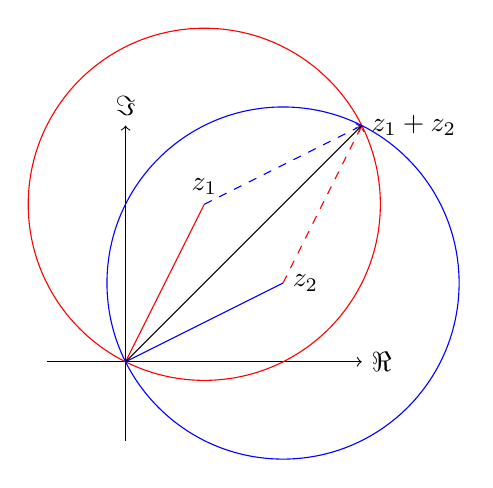
\begin{tikzpicture}
        \draw[->] (-1,0) -- (3,0) node[right] {$\Re$};
        \draw[->] (0,-1) -- (0,3) node[above] {$\Im$};
        \draw (0,0) -- (1,2) node[above] {$z_1$}[red];
        \draw (0,0) -- (2,1) node[right] {$z_2$}[blue];
        \draw (1,2) circle (2.2360679775)[red];
        \draw (2,1) circle (2.2360679775)[blue];
        \draw[dashed,->] (1,2) -- (3,3)[blue];
        \draw[dashed,->] (2,1) -- (3,3)[red];
        \draw (0,0) -- (3,3) node[right] {$z_1 + z_2$};
    \end{tikzpicture}
    \caption{Construction of $z_1 + z_2$}
    \label{Fig.2}
\end{figure}

\begin{corollary}[Subtraction of complex numbers]
    \label{cor:construction_sub}
    \lean{Construction.sub_M_Inf}
    \leanok
    \uses{def:set_of_constructable_points}
    For $z_1, z_2 \in M_{\infty}$ it follows that $z_1 - z_2 \in M_{\infty}$.
\end{corollary}
\begin{proof}
    \uses{lem:construction_neg, lem:construction_add}
    By lemma \ref{lem:construction_neg} and \ref{lem:construction_add} we get $z_1 - z_2 = z_1 + (-z_2) \in M_{\infty}$.
\end{proof}

\begin{corollary}[Construction of parallel lines]
    \label{lem:construction_parallel_lines}
    \lean{Construction.parallel_lines_M_inf}
    \leanok
    \uses{def:set_of_constructable_points, def:set_of_lines, def:parallel}
    For $l \in \mathcal{L(M_{\infty})}$ and $z \in M_{\infty}$ it follows that $\exists l' \in \mathcal{L(M_{\infty})}$ with  $z\in l'$  and  $l\|l'$.
\end{corollary}
\begin{proof}
    \uses{def:line, def:set_of_lines, cor:construction_sub,lem:parallel_by_basis} 
    Let $l$ be a line through $x,y \in \mathcal{M_{\infty}}$ and $z \in \mathcal{M_{\infty}}$.\\
    After corollary \ref{cor:construction_sub} we get $z - x \in \mathcal{M_{\infty}}$ and therfore $z-x + y \in \mathcal{M_{\infty}}$\ref{lem:construction_add}.\\
    Define $l' = \{z, z-x+y\}$, then $l' \in \mathcal{L(M_{\infty})}$ and since a line is defined by two points and we moved them the same distance ($z-x$) $l'$ is parallel to $l$.\ref{lem:parallel_by_basis}
\end{proof}
%2.3.3
%TODO: Comper to mirrowed version
\begin{lemma}[Complex conjugation]
    \label{lem:construction_conj}
    \lean{Construction.conj_M_Inf}
    \leanok
    \uses{def:set_of_constructable_points}
    For $z \in M_{\infty}$ it follows that $\overline{z} \in M_{\infty}$.
\end{lemma}
This construction is taken from \cite{JAN_SCHRÖER:2023}.\\
Draw two circles one with center $0$ and radius $\|z\|$ and a second with center $1$ and radius $\|z-1\|$ and take the intersection of the two circles.\ref{Fig.3}
\begin{proof}
    \uses{def:line, def:circle, lem:icc_M_inf, lem:M_in_M_inf}
    Define $c_1 = \{0,\dist (0, z)\}$ and $c_2 = \{1,\dist (1, z)\}$.\\
    By assumption $0, 1, z \in M_{\infty}$, so $c_1, c_2 \in \mathcal{C(M_{\infty})}$.\\
    \underline{Claim 1}: $\overline{z}$ is in $c_1$.
    \begin{proof}
        The definition of $c_1$ can be written in the following form: $$\{x\in\mathbb{C} \mid \|x-0\| = \dist (0\ z)\}.$$ 
        Using the definition of the distance, we obtain the following result: $$\|0 - \overline{z}\| = \|\overline{z}\| = \|z\| = \dist (0\ z).$$
    \end{proof}
    \underline{Claim 2}: $\overline{z}$ is in $c_2$.
    \begin{proof}
        From the definition of $c_2:=\{x\in\mathbb{C} \mid\|x-1\|=\dist (1\ z)\}$ and the definition of the distance, we can derive the following:
         $$\|1-\overline{z}\| = \|\overline{z}-1\| = \sqrt{(\Re(\overline{z})-1)^2 + \Im(\overline{z})^2} = \sqrt{(\Re(z)-1)^2 + \Im(z)^2} = \|z-1\|=\dist (1\ z).$$
    \end{proof}
    By claim 1 and 2 we get that $\overline{z} \in c_1 \cap c_2$. Futhermore  $\overline{z} $ is in $M_{\infty}$, after lemma \ref{lem:icc_M_inf}.
\end{proof}
\begin{figure}[h]
    \centering
    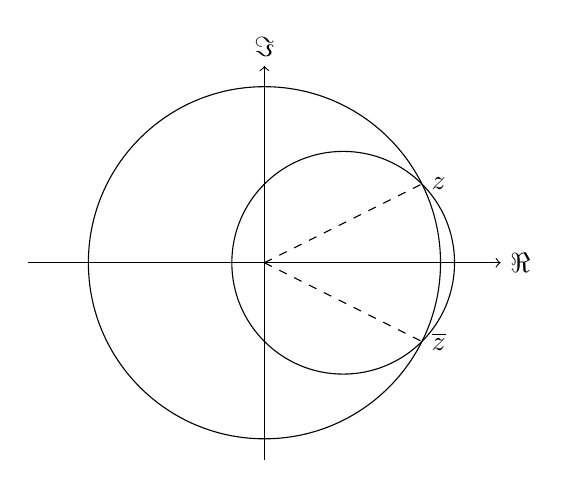
\begin{tikzpicture}
        \draw[->] (-3,0) -- (3,0) node[right] {$\Re$};
        \draw[->] (0,-2.5) -- (0,2.5) node[above] {$\Im$};
        \draw[dashed] (0,0) -- (2,1) node[right] {$z$};
        \draw[dashed] (0,0) -- (2,-1) node[right] {$\overline{z}$};
        \draw (0,0) circle (2.2360679775);
        \draw (1,0) circle (1.4142135624);
    \end{tikzpicture}
    \caption{Construction of $\overline{z}$}
    \label{Fig.3}
\end{figure}


\begin{lemma}[Construction $\imath r\in\mathcal{M}_{\infty}$]
    \label{lem:construction_imath_r}
    \lean{Construction.ir_M_inf}
    \leanok
    \uses{def:set_of_constructable_points}
    For $r \in \mathbb{R}\cap M_{\infty}$ it follows that $\imath\cdot r \in M_{\infty}$.
\end{lemma}
The first step is to construct the imaginary axis, which is achieved by drawing a line, designated as $l$, that passes through two circles with centres at $-1$ and $1$ and radii of $2$. 
The second step is to construct the point, designated as $\imath r$, which is achieved by drawing a circle with a centre at $0$ and a radius of $r$, and taking the intersection with the imaginary axis. (Fig\ref{Fig.4})
\begin{proof}
    \uses{def:line, def:circle, lem:construction_neg, lem:icc_M_inf, lem:ilc_M_inf, lem:M_in_M_inf}
    First we construct the imaginary axis. Define $c_1 = \{-1,2\}$ and $c_2 = \{1,2\}$.\\
    \underline{Claim 1}: $c_1, c_2 \in \mathcal{C(M_{\infty})}$
    \begin{proof}
        By assumption and lemma \ref{lem:construction_neg} we get $-1, 1 \in M_{\infty}$. Using $\dist(-1 1)=2$ we get $c_1, c_2 \in \mathcal{C(M_{\infty})}$, by the definition of the circle.
    \end{proof}
    \underline{Claim 2}: $\imath\sqrt{3}$ and $-\imath\sqrt{3}$ are in $c_1 \cap c_2$.
    \begin{proof}
        Unfolding the definition of $c_1:=\{x\in\mathbb{C} \mid\|x+1\|=2\}$ and $c_2:=\{x\in\mathbb{C} \mid\|x-1\|=2\}$.
        By the definition of the distance we get $\|-\imath\sqrt{3}+1\| = \sqrt{1 + 3} = 2$ and $\|\imath\sqrt{3}-1\| = \sqrt{1 + 3} = 2$.
    \end{proof}
    Now we define $l = \{\imath\sqrt{3}, -\imath\sqrt{3}\}$.\\
    \underline{Claim 3}: $l \in \mathcal{L(M_{\infty})}$
    \begin{proof}
        By claim 2 and \ref{lem:icc_M_inf} we get $\imath\sqrt{3}, -\imath\sqrt{3} \in M_{\infty}$, so $l \in \mathcal{L(M_{\infty})}$.
    \end{proof}
    To get $\imath r$ we define $c = \{0,|r|\}$.\\
    \underline{Claim 4}: $\imath r$ is in $c \cap l$.
    \begin{proof}
        It is clear that $\imath r \in c$. Now using the definition of $l$ and $\lambda = \frac{r}{2\sqrt{3}+\frac{1}{2}}$ we get $(\frac{r}{2\sqrt{3}+\frac{r}{2}})\imath\sqrt{3} + (1-\frac{r}{2\sqrt{3}+\frac{r}{2}})(-\imath\sqrt{3}) = \imath r$. 
    \end{proof}
    Therfore $\imath r \in M_{\infty}$ after lemma \ref{lem:ilc_M_inf}.
\end{proof}
\begin{figure}[h]
    \centering
    \begin{tikzpicture}  
        \draw[->] (-3,0) -- (3,0) node[right] {$\Re$};
        \draw[->] (0,-2.5) -- (0,2.5) node[above] {$\Im$};
        \coordinate[label=-45:$1$] (one) at (1,0);
        \coordinate[label=-135:$-1$] (mone) at (-1,0);
        \fill[black] (one) circle (2pt);
        \fill[black] (mone) circle (2pt);
        \draw[dashed] (one) [carc=110:250:2];
        \draw[dashed] (mone) [carc=70:-70:2];
        \coordinate[label=45:$r$] (r) at (2,0);
        \coordinate[label=135:$\imath r$] (ir) at (0,2);
        \fill[black] (r) circle (2pt);
        \fill[black] (ir) circle (2pt);
        \draw (0,0) [carc=-10:100:2];
    \end{tikzpicture}
    \caption{Construction of $\imath r$}
    \label{Fig.4}
\end{figure}

\begin{corollary}[Construction of $\imath$]
    \label{cor:construction_imath}
    \lean{Construction.imath_M_inf}
    \leanok
    \uses{def:set_of_constructable_points}
    $\imath \in M_{\infty}$.
\end{corollary}
\begin{proof}
    \uses{lem:construction_imath_r, lem:M_in_M_inf}
    By lemma \ref{lem:construction_imath_r} with $r = 1$ and the definition of $\mathcal{M}$ we get $\imath \in M_{\infty}$.
\end{proof}

\begin{lemma}[Construction of real part]
    \label{lem:construction_real}
    \lean{Construction.real_in_M_inf}
    \leanok
    \uses{def:set_of_constructable_points}
    For $z \in M_{\infty}$ it follows that $z.re \in M_{\infty}$.
\end{lemma}
To get the point $z.re$ we draw a line through $z$ and $\overline{z}$. Then $z.re$ is the intersection with the real line, defined by $0$ and $1$.\ref{Fig z.re}
\begin{proof}
    \uses{def:line, } %TODO c_in_C_M, ilc_M_inf, M_M_inf
    Without loss of generality we can assume that $z \in \C\setminus\R$.\\
    Define the lines $l = \{z, \overline{z}\}$ and $l_{\Re} = \{1, 0\}$.\\
    By using Lemma \ref{lem:construction_conj}, they are in $\mathcal{L(M_{\infty})}$.\\
    To show that $z.re \in l \cap l_{\Re}$ we use $t:= 1/2$ for $l$ and $t:= z.re$ for $l_{\Re}$.
\end{proof}
\begin{figure}
    \centering
    \begin{tikzpicture}
        \draw[->] (-0.5,0) -- (5,0) node[right] {$\Re$};
        \draw[->] (0,-3) -- (0,3) node[above] {$\Im$};
        \coordinate[label=135:$z$] (z) at (2,2);
        \coordinate[label=-45:$z.re$] (zre) at (2,0);
        \coordinate[label=135:$\overline{z}$] (oz) at (2,-2);
        \coordinate[label=-135:$0$] (zero) at (0,0);
        \coordinate[label=-90:$1$] (one) at (1,0);
        \fill[black] (z) circle (2pt);
        \fill[black] (zre) circle (2pt);
        \fill[black] (oz) circle (2pt);
        \fill[black] (one) circle (1pt);
        \fill[black] (zero) circle (1pt);
        \draw (z) -- (oz);
    \end{tikzpicture}
    \caption{Construction of $z.re$}
    \label{Fig z.re}
\end{figure}

\begin{lemma}[Construction of imaginary part]
    \label{lem:construction_imag}
    \lean{Construction.im_in_M_inf,Construction.i_z_imp_z_in_M_inf}
    \leanok
    \uses{def:set_of_constructable_points}
    For $z \in M_{\infty}$ it follows that $z.im \in M_{\infty}$.
\end{lemma}
To get the point $z.im$ we draw a line through $z$ and $z-1$. Now we get $\imath \cdot z.im$ by taking the intersection with the imaginary line, defined by $0$ and $\imath$. To get $z.im$ draw a circle trough $\imath \cdot z.im$ and take the intersection with the real line.\ref{Fig z.im}

\begin{proof}
    \uses{def:line, def:circle,}%TODO c_in_C_M, ilc_M_inf, M_M_inf
    Define the lines $l = \{z, z-1\}$ and $l_{\Im} = \{\imath, 0\}$.\\
    Now it is analog to the proof of lemma \ref{lem:construction_real}, that $z.im \cdot \imath  \in l \cap l_{\Im}$. 

    Now we can project $z.im \cdot \imath$ on the real axis by drawing a circle with center $0$ and radius $\|z.im\|$ and taking the intersection with the real axis.
\end{proof}
\begin{figure}
    \centering
    \begin{tikzpicture}
        \draw[->] (-1,0) -- (4,0) node[right] {$\Re$};
        \draw[->] (0,-1) -- (0,4) node[above] {$\Im$};
        \coordinate[label=90:$z$] (z) at (2,3);
        \coordinate[label=-45:$z.im$] (zim) at (3,0);
        \coordinate[label=90:$z-1$] (z1) at (1,3);
        \coordinate[label=-135:$\imath\cdot z.im$] (izim) at (0,3);
        \coordinate[label=-135:$0$] (zero) at (0,0);
        \coordinate[label=180:$\imath$] (i) at (0,1);
        \coordinate[label=-90:$1$] (one) at (1,0);
        \fill[black] (z) circle (2pt);
        \fill[black] (izim) circle (2pt);
        \fill[black] (zim) circle (2pt);
        \fill[black] (z1) circle (2pt);
        \fill[black] (i) circle (1pt);
        \fill[black] (zero) circle (1pt);
        \fill[black] (one) circle (1pt);
        \draw (-0.5,3) -- (3.5,3);
        \draw (0,0) [carc=-30:120:3];
    \end{tikzpicture}
    \caption{Construction of $z.im$}
    \label{Fig z.im}
\end{figure}

\begin{corollary}[$z \in M_{\infty} \Rightarrow z.re, z.im \in M_{\infty}$]
    \label{cor:z_iff_re_im_M_inf}
    \lean{Construction.z_iff_re_im_M_inf}
    \leanok
    \uses{def:set_of_constructable_points}
    For $z \in \C$. $z$ is in $M_{\infty}$ if and only if $z.re, z.im \in M_{\infty}$.
\end{corollary}
\begin{proof}
    \uses{lem:construction_real, lem:construction_imag, lem:construction_add, lem:construction_imath_r}
    "$\Rightarrow$:" If $z \in M_{\infty}$ then $z.re, z.im \in M_{\infty}$ after lemma \ref{lem:construction_real} and \ref{lem:construction_imag}.\\
    "$\Leftarrow$:" If $z.re, z.im \in M_{\infty}$ then $z.re + \imath z.im \in M_{\infty}$ after lemma \ref{lem:construction_add} and lemma \ref{lem:construction_imath_r}.
\end{proof}

\begin{lemma}[Multiplication of positve real numbers]
    \label{lem:construction_mul}
    \lean{Construction.ab_in_M_inf}
    \leanok
    \uses{def:set_of_constructable_points}
    For $a, b \in M_{\infty}\cap\R$ it follows that $a \cdot b \in M_{\infty}$.
\end{lemma}
This construction is taken from \cite{cox2012galois}.\\
To get the point $a\cdot b$ we draw a line trough $a$ and $\imath$ and a parallel line through $\imath b$. The intersection of the second line with the real axis is $a\cdot b$.\ref{Fig.5} 
\begin{proof}
    \uses{def:line, def:set_of_lines, lem:ill_M_inf, lem:construction_imath_r, cor:construction_imath, lem:construction_add, cor:construction_sub}
    Define the three lines $l = \{a+\imath b - \imath, \imath b\}$ and $l_{\Re} = \{1,0\}$.\\
    \underline{Claim 1}: $l \in \mathcal{L(M_{\infty})}$
    \begin{proof}
        By assumption $b \in M_{\infty}$ so after Lemma \ref{lem:construction_imath_r} $\imath b \in M_{\infty}$. Futhermore $l_2 \in \mathcal{L(M_{\infty})}$ after Claim 1 and Lemma \ref{lem:construction_parallel_lines}.
    \end{proof}
    \underline{Claim 2}: $l_{\Re} \in \mathcal{L(M_{\infty})}$
    \begin{proof}
        By assumption $0, 1 \in M_{\infty}$, so $l_{\Re} \in \mathcal{L(M_{\infty})}$.
    \end{proof}
    To show that $a\cdot b \in M_{\infty}$ we need to show that $l \cap l_{\Re} \in M_{\infty}$\ref{lem:ill_M_inf}. That $ab \in l_{\Re} \cap l$ is clear after definition $t=ab$. For $ab \in l$ we use $t=b$ and get $t(a+\imath b - \imath) + (1-t)\imath b  \stackrel{t:=b}{=}ba + \imath b^2 -\imath b + \imath b -\imath b^2 = a\cdot b$.
\end{proof}
\begin{remark}
    This construction uses parallel lines, but it is not needed for the proof of the lemma.
\end{remark}
\begin{figure}
    \centering
    \begin{tikzpicture}
        \draw[->] (-0.5,0) -- (5,0) node[right] {$\Re$};
        \draw[->] (0,-0.5) -- (0,3) node[above] {$\Im$};
        \coordinate[label=135:$\imath$] (i) at (0,1);
        \coordinate[label=-90:$a$] (a) at (2,0);
        \coordinate[label=135:$\imath b$] (ib) at (0,2);
        \coordinate[label=-90:$ab$] (ab) at (4,0);
        \fill[black] (i) circle (2pt);
        \fill[black] (a) circle (2pt);
        \fill[black] (ib) circle (2pt);
        \fill[black] (ab) circle (2pt);
        \draw (a) -- (i);
        \draw (ib) -- (ab);
    \end{tikzpicture}
    \caption{Construction of $z_1 \cdot z_2$}
    \label{Fig.5}
\end{figure}

\begin{corollary}[Multiplication of complex numbers]
    \label{cor:construction_mul_complex}
    %\lean{mul_in_M_inf}
    %\leanok
    \uses{def:set_of_constructable_points}
    For $z_1, z_2 \in M_{\infty}$ it follows that $z_1 \cdot z_2$ in $M_{\infty}$.
\end{corollary}
\begin{proof}
    \uses{lem:construction_mul, lem:construction_add, cor:construction_sub, lem:construction_real, lem:construction_imag}
    Let $z_1 = a + \imath b$ and $z_2 = c + \imath d$. Then $$z_1 \cdot z_2 = (a + \imath b) \cdot (c + \imath d) = (a \cdot c - b \cdot d) + \imath (a \cdot d + b \cdot c).$$
    By combining the Lemmas \ref{lem:construction_mul}, \ref{lem:construction_add}, \ref{cor:construction_sub}, \ref{lem:construction_real} and \ref{lem:construction_imag} we get that $z_1 \cdot z_2 \in M_{\infty}$.
\end{proof}

\begin{lemma}[Invers of a pos real number]
    \label{lem:construction_inv}
    \lean{Construction.ainv_in_M_inf}
    \leanok
    \uses{def:set_of_constructable_points}
    If $a \in M_{\infty}\cap\R$, then $a^{-1}$ is in  $M_{\infty}$.
\end{lemma}

This can be constructed analog to the multiplication of positve real numbers. 
Using the fact that $a\cdot a^{-1} = 1$.
Draw a line through $1$ and $\imath a$ and a parallel line through $\imath$. 
The intersection of the second line with the real axis is $a^{-1}$. (Fig. \ref{Fig.6})
\begin{proof}
    \uses{def:line, def:set_of_lines, lem:ill_M_inf, lem:construction_imath_r, cor:construction_imath, lem:construction_add, cor:construction_sub}
    The proof is analogous to that of Lemma \ref{lem:construction_mul}. It requires only two lines: $l = \{1 - \imath z + \imath, \imath\}$ and $l_{\Re} = \{1,0\}$.\\
    With  out loss of generality we can assume that $a \ne 0$.\\
    The fact that they are in $\mathcal{L(M_{\infty})}$ follows analog to the proof of Lemma \ref{lem:construction_mul}.\\ 
    Thus we have just to show that $z^{-1} \in l$, i.e. $\exists t: t  (1 - \imath a + \imath) + (1 - t)  I = a^{-1}$ $$t  (1 - \imath a + \imath) + (1 - t)  \imath \stackrel{t:=a^{-1}}{=}  a^{-1} - a^{-1} \imath a + a^{-1}\imath + \imath - a^{-1}\imath = a^{-1}.$$
    The rest follows analog.
\end{proof}
\begin{figure}
    \centering
    \begin{tikzpicture}
        \draw[->] (-1,0) -- (2,0) node[right] {$\Re$};
        \draw[->] (0,-1) -- (0,3) node[above] {$\Im$};
        \coordinate[label=135:$\imath$] (i) at (0,1);
        \coordinate[label=-90:$1$] (1) at (1,0);
        \coordinate[label=135:$\imath a$] (ia) at (0,2);
        \coordinate[label=-90:$a^{-1}$] (ainv) at (0.5,0);
        \fill[black] (i) circle (2pt);
        \fill[black] (1) circle (2pt);
        \fill[black] (ia) circle (2pt);
        \fill[black] (ainv) circle (2pt);
        \draw (1) -- (ia);
        \draw (i) -- (ainv);
    \end{tikzpicture}
    \caption{Construction of $z^{-1}$}
    \label{Fig.6}
\end{figure}

\begin{corollary}[Invers of a complex number]
    \label{cor:inv_M_inf}
    \lean{Construction.inv_M_inf, Construction.z_inv_eq}
    \leanok
    \uses{def:set_of_constructable_points}
    If $z \in M_{\infty}$, then $z^{-1}$ is in  $M_{\infty}$.
\end{corollary}
\begin{proof}
    \uses{lem:construction_inv, lem:construction_mul, cor:construction_sub, lem:construction_real, lem:construction_imag, lem:construction_add}
    For $z \in M_{\infty}$ we can write $z = a + \imath b$ with $a, b \in \R$. Then
    $$z^{-1} = \frac{1}{z} = \frac{\overline{z}}{z\overline{z}} = \frac{a - \imath b}{a^2+b^2}= (a - \imath b) \cdot (aa+bb)^{-1}.$$
    It is now possible to combine the lemmas for addition \ref{lem:construction_add}, subtraction \ref{cor:construction_sub}, multiplication \ref{cor:construction_mul_complex} 
    and the corollary for the inverse of a positive real number \ref{lem:construction_inv} with the part concerning the existence of real and imaginary components \ref{cor:z_iff_re_im_M_inf} in order to conclude that $z^{-1} \in M_{\infty}$.
\end{proof}


\begin{lemma}[Angle in $M_{\infty}$]
    \label{lem:angle_M_inf}
    \uses{def:set_of_constructable_points}
    \lean{Construction.angle_M_inf}
    \leanok
    If $0 \ne z = r\cdot e^{\imath\alpha} \in M_{\infty}$, then $e^{\imath\alpha} \in  M_{\infty}$.
\end{lemma}
For the constrution we draw a line through $0$ and $z$ and take the intersection with the unit circle. \ref{Fig.angle}

\begin{proof}

    Let $l$ be a line through $0$ and $z$ and $c$ be the unit circle. Then $l \cap c = \{e^{\imath\alpha}\}$.
    The rest follows from the construction of the intersection of a line and a circle\ref{lem:icc_M_inf}.
\end{proof}

\begin{figure}[h]
    \centering
    \begin{tikzpicture}
        \draw[->] (-0.5,0) -- (4,0) node[right] {$\Re$};
        \draw[->] (0,-0.5) -- (0,3) node[above] {$\Im$};
        \coordinate[label=-135:$0$] (zero) at (0,0);
        \coordinate[label=-135:$1$] (one) at (1,0);
        \coordinate[label=135:$z$] (z) at (3,2);
        \coordinate[label=90:$e^{\imath\alpha}$] (ea) at (0.8321,0.5547);
        \fill[black] (zero) circle (1pt);
        \fill[black] (one) circle (2pt);
        \fill[black] (z) circle (2pt);
        \fill[black] (ea) circle (2pt);
        \draw (zero) -- (z);
        \draw (zero) [carc=-20:110:1];
    \end{tikzpicture}
    \caption{Construction of $e^{\imath\alpha}$}
    \label{Fig.angle}
\end{figure}

\begin{corollary}[Midpoint in $M_{\infty}$]
    \label{cor:Construction.midpoiont}
    \uses{def:set_of_constructable_points}
    \lean{Construction.midpoiont}
    \leanok
    If $z_1, z_2 \in M_{\infty}$, then $\frac{z_1 + z_2}{2} \in  M_{\infty}$.
    
\end{corollary}

\begin{proof}
    \uses{lem:construction_add, lem:construction_mul, lem:construction_inv}
    Combeing the lemmas for addition\ref{lem:construction_add}, multiplication\ref{cor:construction_mul_complex} and the invers of a complex number\ref{cor:inv_M_inf} we get that $\frac{z_1 + z_2}{1+1} \in M_{\infty}$.
\end{proof}

\begin{lemma}[Halving of an angle]
    \label{lem:Construction.angle_half_M_inf}
    \uses{def:set_of_constructable_points}
    \lean{Construction.angle_half_M_inf}
    \leanok
    For $\alpha \in [0,2\pi)$, if $e^{\imath\alpha} \in M_{\infty}$, then $e^{\imath\frac{\alpha}{2}} \in  M_{\infty}$.
\end{lemma}
\begin{proof}
    \uses{lem:angle_M_inf, lem:icc_M_inf}
    For $\alpha \ne 0 \ne \pi$ we take the intersection of the unit circle with the line through $0$ and and the mipiont of $e^{\imath\alpha}$ and $1$. 
    
    For $\alpha = 0$ we get $e^{\imath\frac{\alpha}{2}} = 1$ and for $\alpha = \pi$ we get $e^{\imath\frac{\alpha}{2}} = \imath$.
    
\end{proof}

\begin{lemma}[Construction of radius]
    \label{lem:construction_radius}
    \uses{def:set_of_constructable_points}
    If $z = r\cdot e^{\imath\alpha} \in M_{\infty}$, then $r \in  M_{\infty}$.
\end{lemma}
\begin{remark}
    The radius is the distance from $0$ to $z$, which is the same as $\|z\|$.
\end{remark}
We get the radius by taking the intersection of the real axis with a circle in zero with radius $\dist (0,z)$. \ref{Fig.radius}
\begin{proof}
    We use the fact that $r = \|z\| = \sqrt{\Re(z)^2 + \Im(z)^2}$. Since we have spilt $r$ in already constructed parts, we get that $r \in M_{\infty}$.
\end{proof}

\begin{figure}[h]
    \centering
    \begin{tikzpicture}
        \draw[->] (-0.5,0) -- (4,0) node[right] {$\Re$};
        \draw[->] (0,-0.5) -- (0,4) node[above] {$\Im$};
        \coordinate[label=-135:$0$] (zero) at (0,0);
        \coordinate[label=-135:$1$] (one) at (1,0);
        \coordinate[label=90:$z$] (z) at (3,2);
        \coordinate[label=-135:$r$] (r) at (3.6056,0);
        \fill[black] (zero) circle (2pt);
        \fill[black] (one) circle (1pt);
        \fill[black] (z) circle (2pt);
        \fill[black] (r) circle (2pt);
        \draw (zero) -- (z);
        \draw (zero) [carc=-10:100:3.6056];
    \end{tikzpicture}
    \caption{Construction of $r = \|z\|$}
    \label{Fig.radius}
\end{figure}

\begin{lemma}[Root of pos real numer]
    \label{lem:pos_real_root}
    \lean{Construction.one_real_root, Construction.zero_real_root_M_inf}
    If $r \in M_{\infty}\cap\R_{\ge 0}$, then $\sqrt{r}$ is in  $M_{\infty}$.
\end{lemma}

This construction is taken from  \cite{JAN_SCHRÖER:2023}.\\
Draw a circle trough $0$ and $r$ and a line through $1$ parallel to the imaginary axis. Project the intersection to the real axis, using a circle with center $0$ and you get $\sqrt{r}$. (Fig. \ref{Fig.root})
\begin{proof}
    \uses{def:line, def:circle, lem:icc_M_inf, lem:M_in_M_inf} %TODO add rest of dependencies   
Without loss of generality we can assume that $r \ge 1$. 
Otherwise we can use the fact that $\sqrt{r} = \frac{1}{\sqrt{r^{-1}}}$.
The initial step is to define the following lines and circles:
\begin{itemize}
    \item [$l_1$] $:= \{z_1 :=1; z_2 := \imath + 1\}$
    \item [$l_{\Re}$] $:= \{z_1:=0; z_2:= 1\}$
    \item [$c_1$] $:= \{\text{center}:= \frac{r}{2}; \text{radius} := \dist (0,\frac{r}{2})\}$
    \item [$c_2$] $:= \{\text{center}:= 0; \text{radius} := \dist (0,\sqrt{r})\}$
\end{itemize}
It can be observed that both $l_1$ and $l_{\Re}$ are elements of $L(M)$, and that $c_1$ is an element of $C(M)$. 
Furthermore, it can be demonstrated that the $\sqrt{r}$  is an element of $l_{\Re} \cap c_2$. 
Consequently, the only remaining step is to show that $c_2$ is an element of $C(M)$, which is equivalent to proving that there exists a $z$ in $M_{\infty}$ that is also an element of $c_2$. 
This is possible since $0$ is an element of $M_{\infty}$.\\
\underline{Claim}: There exists a $z \in l_1 \cap c_1$, such that $z \in c_2$.
\begin{proof}
    In accordance with the theorem of Pythagoras, it can be demonstrated that$z= 1 \pm \imath \sqrt{r-1}$.
    A further application of the Pythagorean theorem yields the following result: 
    $$\dist (0,z) \overset{z= 1 + \imath \sqrt{r-1}}{=} \sqrt{1^2 + (\sqrt{r-1})^2} = \sqrt{1 + r - 1} = \sqrt{r} = \dist (0,\sqrt{r}).$$
\end{proof}
Therefore, it can be concluded that $\sqrt{r}$ is also constructible.

\end{proof}
\begin{figure}[h]
    \centering
    \begin{tikzpicture}
        \draw[->] (-1,0) -- (7,0) node[right] {$\Re$};
        \draw[->] (0,-1) -- (0,4) node[above] {$\Im$};
        \coordinate[label=-135:$0$] (zero) at (0,0);
        \coordinate[label=-90:$1$] (one) at (1,0);
        \coordinate[label=-45:$r$] (r) at (6,0);
        \coordinate[label=-90:$\frac{r}{2}$] (r2) at (3,0);
        \coordinate[label=135:] (sqrt1) at (1,2.2360679775);
        \coordinate[label=135:$\sqrt{r}$] (sqrt) at (2.4494897428,0);
        \fill[black] (zero) circle (1pt);
        \fill[black] (one) circle (2pt);
        \fill[black] (r) circle (2pt);
        \fill[black] (r2) circle (2pt);
        \fill[black] (sqrt1) circle (2pt);
        \draw (r2) [carc=-10:190:3];
        \draw (zero) [carc=-10:80:2.4494897428];
        \draw (one) -- (sqrt1);
        \fill[red] (sqrt) circle (3pt);
    \end{tikzpicture}
    \caption{Construction of $\sqrt{r}$}
    \label{Fig.root}
\end{figure}

\begin{corollary}[Square root of a complexnumber]
    \label{cor:root_M_inf}
    \uses{def:set_of_constructable_points}
    If $z \in M_{\infty}$, then $\sqrt{z}$ is in  $M_{\infty}$.
\end{corollary}
\begin{proof}
    $z = r \cdot e^{\imath \alpha}$ with $r \in \R_{\ge 0}$ and $\alpha \in \R$. Then $\sqrt{z} = \sqrt{r} \cdot e^{\imath \frac{\alpha}{2}}$.
    Now we can use Lemma \ref{lem:construction_radius} and Lemma \ref{lem:pos_real_root} to get that $\sqrt{z} \in M_{\infty}$. For $e^{\imath \frac{\alpha}{2}}$ we can combine Lemma \ref{lem:angle_M_inf} and Lemma \ref{lem:Construction.angle_half_M_inf}. Now we get that $\sqrt{z} \in M_{\infty}$, after Lemma \ref{lem:construction_mul}.

\end{proof}




%2.5
% \begin{lemma}
%   \label{lem:sqrt_in_M_inf}
%   For $M\subseteq \mathbb{C}$ with $0,1 \in M$. If $z$ the $M_{\infty}$, then is $\sqrt{z} \in M_{\infty}$.
% \end{lemma}
% \begin{proof}
%    Let $z = r \exp(\imath \alpha) \in M_{\infty}$, whitout loss of generality we can assume that $r \ne 0$. 
%    Lemma \ref{THM:M_inf_properties}(iv) implies that $r, \exp(\imath \alpha) \in M_{\infty}$. By combining construction \ref{lem:Construction.angle_half_M_inf},
%    which states that $\exp(\imath \alpha / 2) \in M_{\infty}$ and construction \ref{construction_sqrt_pos_real},
%    that gives us that $\sqrt{r} \in M_{\infty}$, we get that $$\sqrt{z} = \sqrt{r} \exp(\imath \alpha / 2) \in M_{\infty}.$$
% \end{proof}
